\documentclass[12pt, a4paper]{scrreprt}
\title{KernowMiner Design Bible}
\subtitle{Version 0.1}
\usepackage{caption}
\date{\today}
\usepackage{graphicx}
\usepackage{csquotes}

\setcounter{tocdepth}{2}
\setcounter{secnumdepth}{-1}

\begin{document}
	
\begin{titlepage}
	\centering
	\vspace*{\fill}
	{\Huge\bfseries KernowMiner Design Bible\par}
	\vspace{0.5em}
	{\Large Version 0.1.1\par}
	\vspace{1em}
	{\large \today\par}
	\vspace{2em}
	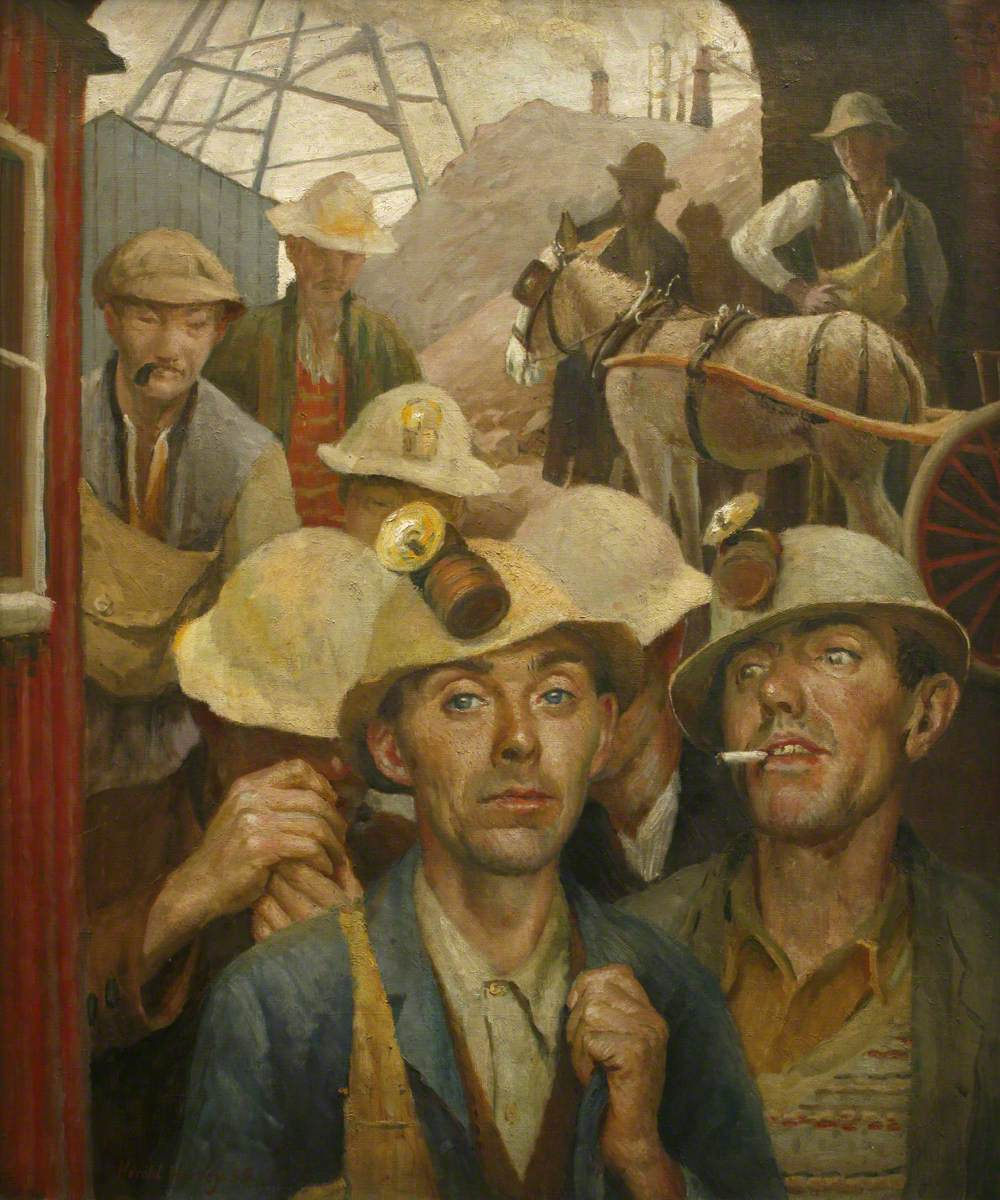
\includegraphics[width=0.9\linewidth]{ImageRefs/StJustTinMiners}
	\captionof*{figure}{'St Just Tin Miners' Harold Harvey, 1935}
	\vspace*{\fill}
\end{titlepage}
	\tableofcontents
	\part{Narrative}
	\chapter{Broad Concepts}
	\section{Ludonarrative} 
	The Ludonarrative (from Latin `ludos' meaning `game') is the narrative of interaction, the interlocking motion of mechanical systems and the narrative frameworks contextualising them that produce the unique idiosyncratic experience of play. The core goal of this project is to tailor this arrangement of systems and narrative context in a way that explores the kinds of social transformation historically driven by the accelerating logic of techno-capital in one of its birthplaces in the Cornish countryside. To put the player in the position of the mine captain. A figure that sits at a sort of crossroad between the rapidly emerging industrial international market and the communities and families that rely on the operations of the mine to live. The captain must navigate these conflicts of interest with careful regard for the responsibilities vested in them, by both the communities and financial structures that they serve, bearing witness to the immense physical and social upheaval this process historically involved.
	\pagebreak
	\section{Themes}
	The transformation of people and environment by alien forces beyond their control. The metamorphosis of the moral framework of labour in its relationship to faith, the land, and the means of production.
	\blockquote[Karl Marx, \emph{Fragment On Machines} (1857--58)][.]{
	The worker's activity, reduced to a mere abstraction of activity, is determined and regulated on all sides by the movement of the machinery, and not the opposite. The science which compels the inanimate limbs of the machinery, by their construction, to act purposefully, as an automaton, does not exist in the worker's consciousness, but rather acts upon him through the machine as an alien power, as the power of the machine itself. (...) The production process has ceased to be a labour process in the sense of a process dominated by labour as its governing unity. Labour appears, rather, merely as a conscious organ, scattered among the individual living workers at numerous points of the mechanical system; subsumed under the total process of the machinery itself, as itself only a link of the system, whose unity exists not in the living workers, but rather in the living (active) machinery, which confronts his individual, insignificant doings as a mighty organism. In machinery, objectified labour confronts living labour within the labour process itself as the power which rules it; a power which, as the appropriation of living labour, is the form of capital. The transformation of the means of labour into machinery, and of living labour into a mere living accessory of this machinery, as the means of its action, also posits the absorption of the labour process in its material character as a mere moment of the realization process of capital}
	\pagebreak
	\section{Stories}
	\subsection{Local}
	Trevithick/Watt dispute, Rise of methodism, Abolition movement,Fall of the Prices , Rise of the Bolithos, The consequences of enclosure, The Expansion of the railroads, smuggling/skullduggery, Penzance Natural History and Antiquarian Society/focus on Ancient sites, Royal Geological Society of Penzance/birth of geology
	\subsection{National}
	Hungry 40s, Napoleonic wars, global price fluctuations from other international events
	\subsection{Events}
	\section{Compromises}
	Time compressions, gaps in the record that necessitate interpretation
	\chapter{Timeline}
	\part{Technical}
	\chapter{Big Picture}
	The game is ultimately going to take the form of three conceptual components, the mine, the community, and the rest of the world. Each of these will be connected to one another through the underlying simulation which will put the fate of two of these components in the hands of the player, one indirectly, and the other through the UI system. The two primary cycles of the game will be daily and weekly with monthly and seasonal cycles also playing an important, but higher level role. The weekly cycle will be used to give directives for the mine, then in the daily operations different actions may be necessary to continue or optimise operations, reactions to events, shuffling of labour allocation to maximise profitability, etc. 
	
	The goal of the current phase of development is getting the game in a state to model a year of simplified gameplay, this process should greatly inform the challenges of further extending the scale and complexity of the simulation.
	\section{Architecture}
	To promote maintainability and extensibility the game follows a high level model-view-controller pattern. Frontend code is concerned with the implementation details of user interfacing and visual representation, the components of the frontend that need to interact with the underlying model do so through the orchestrator's APIs, and state changes flow from the model to the frontend through the orchestrator's signal handling. Backend code is passive, and primarily concerned with recording the program's state and acting as a source of truth for the other layers. A core goal of this approach is to maintain a 'plug and play' capacity so that both the underlying simulation(s) and the frontend interface can be heavily modified or entirely swapped out without having to modify the entire system, abstracting changes behind the facade provided by the orchestrator.
	\chapter{Frontend}
	\section{Camera}
	A Godot Camera2D node that can pan and zoom around the dimensions of the background TextureRect by interpreting unhandled scroll and MMB inputs. Scrolling zooms the camera by a defined multiplier and panning uses the delta in mouse position while holding MMB to proportionally move the camera a number of pixels then applies further decaying motion proportional to the acceleration of that delta. The parent node of both the background TextureRect and the Camera contains a connection that automatically updates the dimensions of the camera's enforced boundaries whenever the dimensions of the background change.
	\subsubsection*{Camera node custom parameters:}
	\begin{itemize}
		\item Zoom Step: 1.1
		\item Max Zoom: 4.0
		\item Drag Sensitivity: 1
		\item Slide Friction: 2000
		\item Slide Min Speed: 40
	\end{itemize}
	\section{Backgrounds}
	Backgrounds are large TextureRect nodes from which the visible boundaries of the game are derived, they primarily serve as visual context for buttons or other gameplay elements. They also have some dynamic cosmetic behaviours related to the time of day, and will in the future react to many other conditions in the game state. The backgrounds as they exist now are placeholders and represent concepts that have been dropped in favour of a slightly different approach. With the above and below ground sections being different backgrounds rather than parts of one larger background. This allows a more practical visual abstraction between layers that the full vertical slice cross section approach in the placeholder wouldn't allow.
	\subsection{Cosmetic Behaviours}
	The way this currently works is a proof of concept that will be reworked to allow for better flexibility in the future. Currently it works by creating a resource that associates a background texture with an integer between 0 and 23, and then listens for the hourly signal fired by the game clock to know when to swap textures. In the future i want to make the sky transparent and have a separate resource for handling things like a moving sky, moon phases, or other astral events. The system that exists now for the daycycle can be adapted for seasonal cycles, or arbitrary events that change the background.
	\subsection{Lighting}
	This is something i'd expect to implement alongside a refinement pass of the mine gameplay, which at this stage is still itself entirely conceptual. I would very much like to implement some simple 2D lighting, both for the day/night cycle and to make the subterranean parts of the background more dynamic. The only way i can see this working currently is by dividing a portion of the visual content of the backgrounds into `foreground' and `background' layers to implement coloured lighting and shadowcasting.
	\subsection{Maps}
	Not yet implemented, likely to begin to take shape alongside the ledger. Maps of the Penwith peninsula, Cornwall, Britain, and the world. Each with ways to interact with far off individuals, organisations, and businesses, as well as visualising deals made by the player. As in showing the delivery progress of purchases or deals that the player is a stakeholder in with an Indiana Jones style dotted line on the map, or showing the progress of workers walking to work from the surrounding area.
	\section{Floating UI}
	The interface systems built on the CanvasLayer that move with the Camera.
	\subsection{Topbar}
	\subsubsection{Clock}
	A series of visual buttons that map to functions in the orchestrator's time API for controlling the game's timescale.
	\subsubsection{Widgets}
	Not yet implemented. Icons relating to resource counts or other relevant information, also acting as buttons that connect to the relevant page in the ledger. Could be worthwhile making this sort of relationship structural, and allow the user to modify the order and content of these widgets. Allowing any kind of resource or statistic to have a shortcut added to a limited number of slots akin to the later Anno games, but this is a second-pass goal.
	\subsection{Window System}
	(under development)
	\subsubsection{Ledger}
	This is something that will be implemented just before, and alongside the first pass at the simulation. A management screen documenting everything relevant about the mine with interfaces to modify operating characteristics of the enterprise. Employment, labour allocation, expense and revenue books, etc. Essentially the player's control console. Some kind of third party data modelling module could be exceptionally useful here.
	\subsubsection{Buildings}
	Constituent components of the mine represented by TextureButtons placed relative to a background. The buildings will be associated with entries in the ledger and act as shortcuts to their respective entries. These will contain an interface with a visual representation of the interior of the building beside a control console for that building including relevant operating information, potential upgrades, and employment/labour allocation options.
	\chapter{Backend}
	\section{Simulation}
	\subsection{Clock}
	The clock involves 3 components, a Godot Timer object, an API contained in the orchestrator node, and a record of the clock's state held by the model obfuscated behind the orchestrator. The clock works by the Godot Timer sending a heartbeat signal on a predefined period. This signal increments an accumulator variable and once that variable reaches a predefined threshold the threshold's value is subtracted from the accumulated value and a signal is sent to the clock's state incrementing a time value from which all other denominations of time are derived. This signal also acts as the lowest level 'tick' of the simulation. Timescale is controlled by modulating the amount accumulated per heartbeat, higher timescales can result in remainders from the accumulated value between tick cycles which allows the timescale to be modified in real time without any awkward 'jerks'. Previously the timer would sometimes hang for a noticeable number of milliseconds when switching between timescales as they necessitated starting the tick cycle from the beginning instead of taking the proportion of 'tick progress' recorded by the accumulator and using that as the starting point for the new timescale.
	
	The current functionality of the clock is pretty close to finalised, however there is one last major necessary change. Currently each tick represents a minute of game time which is analogous to a real world second on the lowest speed, however the game is planned to span at least half a century, and running the game with that level of granularity would simply be too slow. For instance at a minute per second, even at 10x speed it would take almost 15 hours for a year to pass, for a game supposed to span 50 years this isn't acceptable, So i think a shift towards the hour as the most granular unit of time for the sake of simulation is worthwhile, if somewhat time consuming.
	subsection{}
	\part{Visuals}
	Leaving this section blank for now, i have some ideas but the only concrete ones relate to implementation details and the place for that is in the technical section, refinement time is needed for other concepts and this is work best done later in development to avoid wasted effort.
	\chapter{Rich Backgrounds}
	\section{Background Images}
	\subsection{Background States}
	\subsection{Background Buttons}
	\section{Sprites}
	\chapter{Floating UI}
	\section{General Style}
	\subsection{Fonts}
	\section{Portraits}
	\section{Building Interiors}
	\section{Events}
	\subsection{Mail}
	\subsection{Popups}
	\section{Ledger}
	\part{References}
	\chapter{Images}
	\chapter{Bibliography}
\end{document}
